\documentclass[tikz,border=2pt]{standalone}
\usepackage{amsmath,amssymb}
\usepackage{pgfplots}
\pgfplotsset{compat=1.18}

\begin{document}
% Three surfaces and their Hessians: a bowl (PSD everywhere: convex), a cap (NSD: concave)
% and a saddle (indefinite: neither).
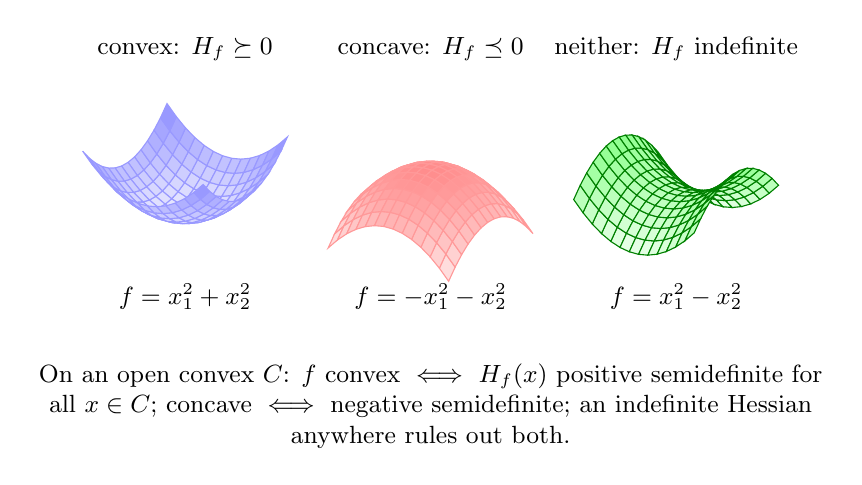
\begin{tikzpicture}
	\begin{axis}[name=p1, view={35}{28}, xmin=-1.3, xmax=1.3, ymin=-1.3, ymax=1.3, zmin=-2.2, zmax=2.4, xtick=\empty, ytick=\empty, ztick=\empty, axis lines=none, width=4.4cm, height=4.2cm, clip=false, title={convex: $H_f\succeq0$}, title style={font=\small}]
		\addplot3[surf, shader=faceted, faceted color=blue!40, colormap={pale}{color=(blue!8) color=(blue!45)}, samples=14, domain=-1.2:1.2, domain y=-1.2:1.2, z buffer=sort] {x^2+y^2-1};
		\node[font=\small, anchor=north, yshift=-8pt] at (axis cs:0,0,-2.3) {$f=x_1^2+x_2^2$};
	\end{axis}
	\begin{axis}[name=p2, at={(p1.east)}, anchor=west, xshift=0.3cm, view={35}{28}, xmin=-1.3, xmax=1.3, ymin=-1.3, ymax=1.3, zmin=-2.2, zmax=2.4, xtick=\empty, ytick=\empty, ztick=\empty, axis lines=none, width=4.4cm, height=4.2cm, clip=false, title={concave: $H_f\preceq0$}, title style={font=\small}]
		\addplot3[surf, shader=faceted, faceted color=red!40, colormap={pale}{color=(red!8) color=(red!45)}, samples=14, domain=-1.2:1.2, domain y=-1.2:1.2, z buffer=sort] {1-x^2-y^2};
		\node[font=\small, anchor=north, yshift=-8pt] at (axis cs:0,0,-2.3) {$f=-x_1^2-x_2^2$};
	\end{axis}
	\begin{axis}[name=p3, at={(p2.east)}, anchor=west, xshift=0.3cm, view={35}{28}, xmin=-1.3, xmax=1.3, ymin=-1.3, ymax=1.3, zmin=-2.2, zmax=2.4, xtick=\empty, ytick=\empty, ztick=\empty, axis lines=none, width=4.4cm, height=4.2cm, clip=false, title={neither: $H_f$ indefinite}, title style={font=\small}]
		\addplot3[surf, shader=faceted, faceted color=green!50!black, colormap={pale}{color=(green!8) color=(green!45)}, samples=14, domain=-1.2:1.2, domain y=-1.2:1.2, z buffer=sort] {x^2-y^2};
		\node[font=\small, anchor=north, yshift=-8pt] at (axis cs:0,0,-2.3) {$f=x_1^2-x_2^2$};
	\end{axis}
	\node[anchor=north, align=flush center, text width=10cm, font=\small, yshift=-22pt] at (p2.south) {On an open convex $C$: $f$ convex $\iff$ $H_f(x)$ positive semidefinite for all $x\in C$; concave $\iff$ negative semidefinite; an indefinite Hessian anywhere rules out both.};
\end{tikzpicture}
\end{document}
